\documentclass{standalone}
\usepackage{tikz}
\usetikzlibrary{patterns, positioning}
\usepackage[sfdefault]{ClearSans} %% option 'sfdefault' activates Clear Sans as the default text font
\usepackage[T1]{fontenc}

\begin{document}
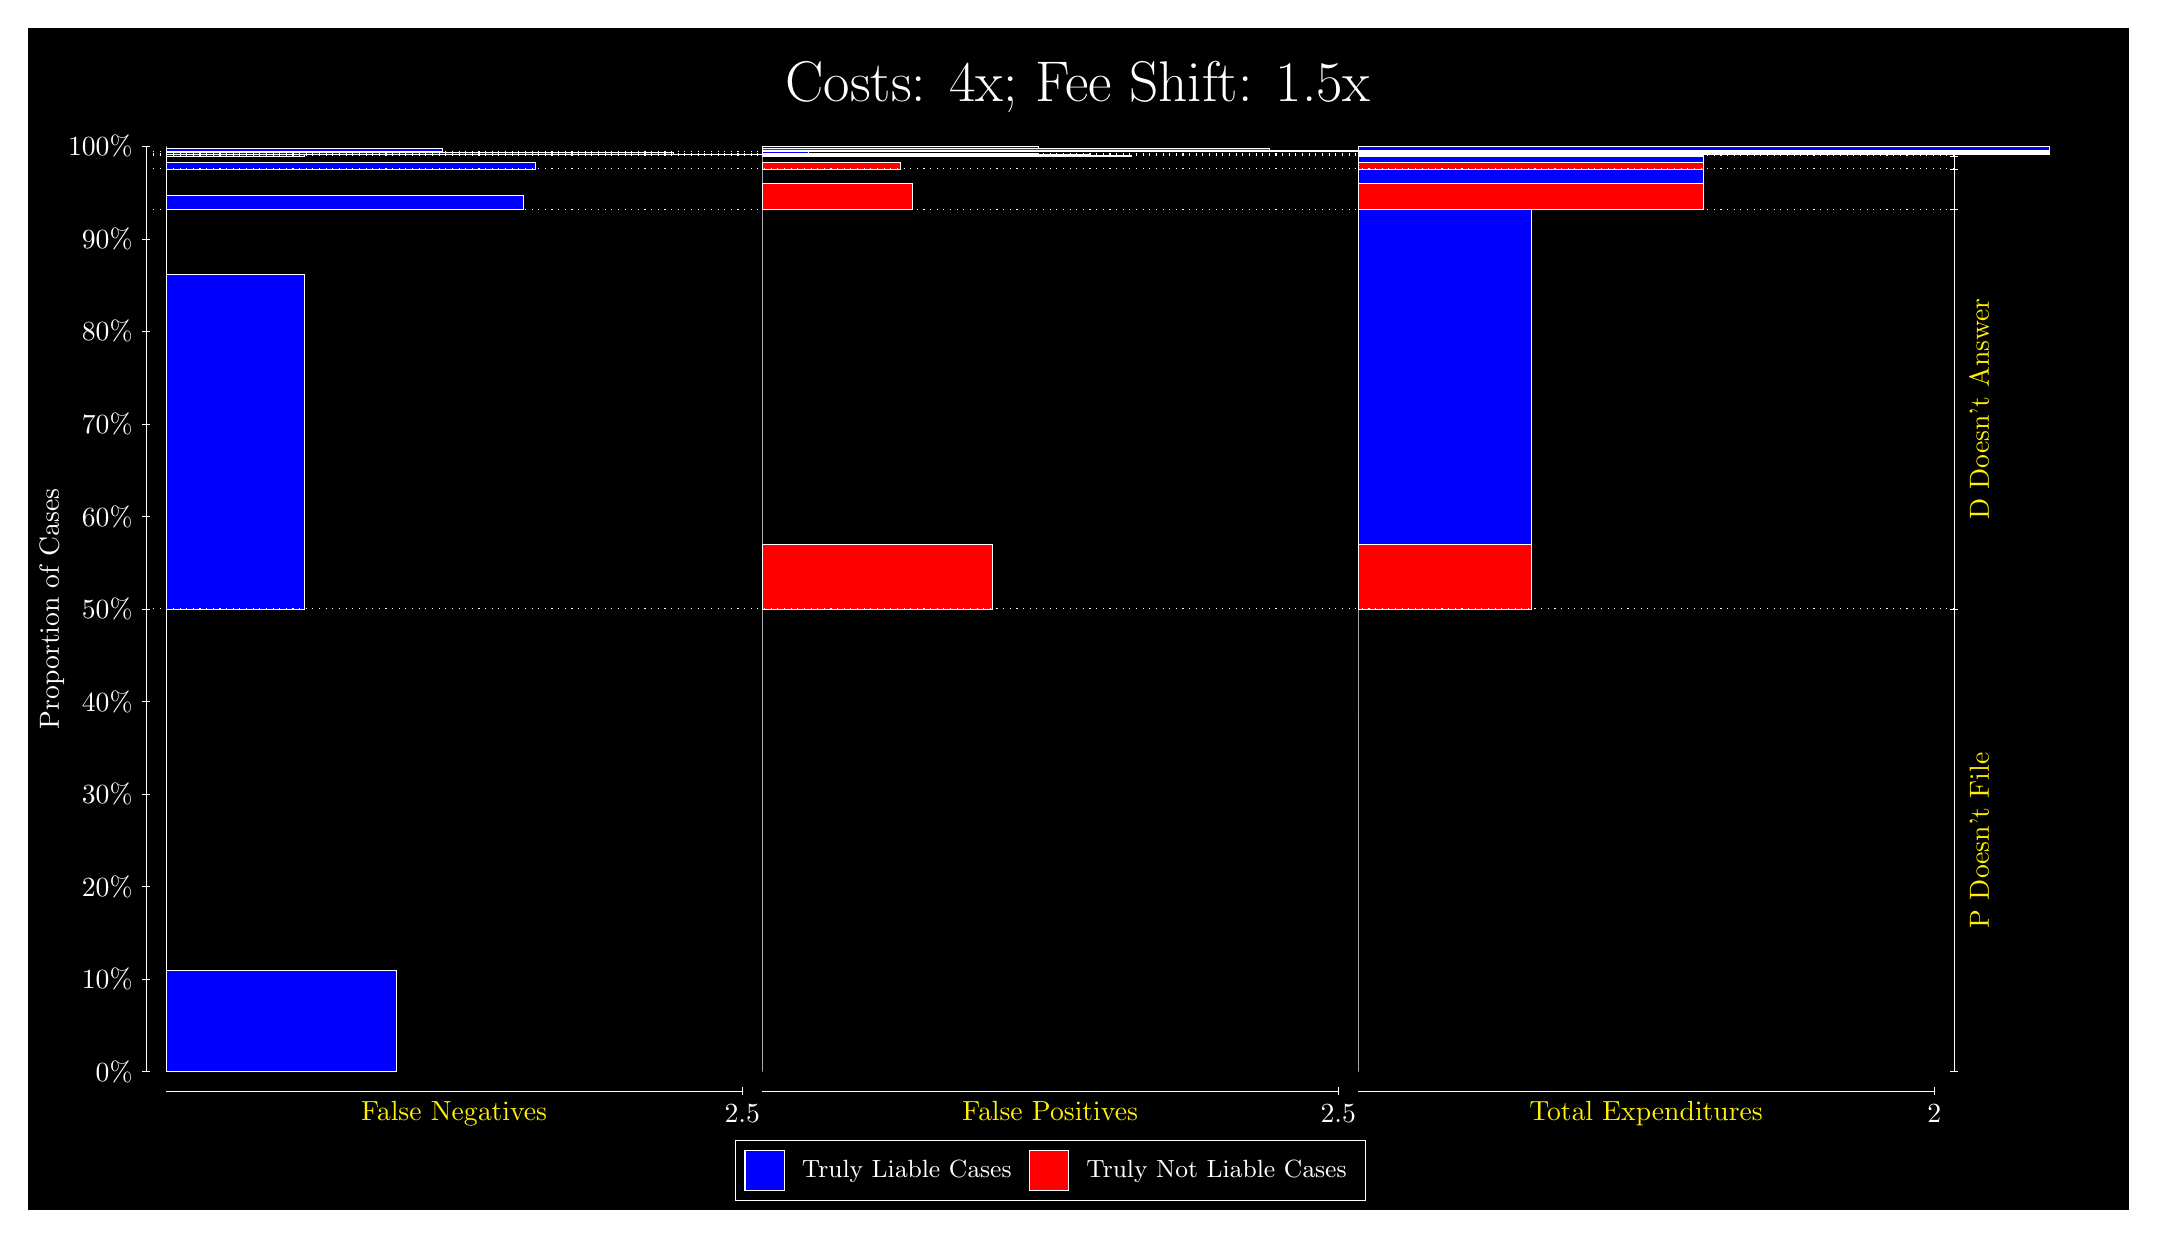
\begin{tikzpicture}
\draw[fill=black] (0,0) rectangle (26.667,15);
\draw[text=white] (0,13.5) rectangle (26.667,15) node[midway] {\huge Costs: 4x; Fee Shift: 1.5x};
\draw[white, very thin] (1.5,1.75) -- (1.5,13.5);
\node[rotate=90, text=white, anchor=center] at (0.3, 7.625) {Proportion of Cases};
\draw[white, very thin] (1.45,1.75) -- (1.55,1.75);
\node[text=white, anchor=east] at (1.45, 1.75) {0\%};
\draw[white, very thin] (1.45,2.925) -- (1.55,2.925);
\node[text=white, anchor=east] at (1.45, 2.925) {10\%};
\draw[white, very thin] (1.45,4.1) -- (1.55,4.1);
\node[text=white, anchor=east] at (1.45, 4.1) {20\%};
\draw[white, very thin] (1.45,5.275) -- (1.55,5.275);
\node[text=white, anchor=east] at (1.45, 5.275) {30\%};
\draw[white, very thin] (1.45,6.45) -- (1.55,6.45);
\node[text=white, anchor=east] at (1.45, 6.45) {40\%};
\draw[white, very thin] (1.45,7.625) -- (1.55,7.625);
\node[text=white, anchor=east] at (1.45, 7.625) {50\%};
\draw[white, very thin] (1.45,8.8) -- (1.55,8.8);
\node[text=white, anchor=east] at (1.45, 8.8) {60\%};
\draw[white, very thin] (1.45,9.975) -- (1.55,9.975);
\node[text=white, anchor=east] at (1.45, 9.975) {70\%};
\draw[white, very thin] (1.45,11.15) -- (1.55,11.15);
\node[text=white, anchor=east] at (1.45, 11.15) {80\%};
\draw[white, very thin] (1.45,12.325) -- (1.55,12.325);
\node[text=white, anchor=east] at (1.45, 12.325) {90\%};
\draw[white, very thin] (1.45,13.5) -- (1.55,13.5);
\node[text=white, anchor=east] at (1.45, 13.5) {100\%};

\draw[white, very thin] (24.457,1.75) -- (24.457,13.5);
\draw[white, very thin] (24.407,1.75) -- (24.507,1.75);
\node[anchor=west] at (24.407, 1.75) {};
\draw[white, very thin] (24.407,7.6251) -- (24.507,7.6251);
\node[anchor=west] at (24.407, 7.6251) {};
\draw[white, very thin] (24.407,12.701) -- (24.507,12.701);
\node[anchor=west] at (24.407, 12.701) {};
\draw[white, very thin] (24.407,13.213) -- (24.507,13.213);
\node[anchor=west] at (24.407, 13.213) {};
\draw[white, very thin] (24.407,13.378) -- (24.507,13.378);
\node[anchor=west] at (24.407, 13.378) {};
\draw[white, very thin] (24.407,13.403) -- (24.507,13.403);
\node[anchor=west] at (24.407, 13.403) {};
\draw[white, very thin] (24.407,13.438) -- (24.507,13.438);
\node[anchor=west] at (24.407, 13.438) {};
\draw[white, very thin] (24.407,13.5) -- (24.507,13.5);
\node[anchor=west] at (24.407, 13.5) {};

\draw[white, very thin, fill=blue] (1.75,1.75) rectangle (4.6775,3.0357);
\draw[white, very thin, fill=red] (1.75,3.0357) rectangle (1.75,7.6251);
\draw[white, very thin, fill=blue] (1.75,7.6251) rectangle (3.5065,11.879);
\draw[white, very thin, fill=red] (1.75,11.879) rectangle (1.75,12.701);
\draw[white, very thin, fill=blue] (1.75,12.701) rectangle (6.2877,12.877);
\draw[white, very thin, fill=red] (1.75,12.877) rectangle (1.75,13.213);
\draw[white, very thin, fill=blue] (1.75,13.213) rectangle (6.4341,13.293);
\draw[white, very thin, fill=red] (1.75,13.293) rectangle (1.75,13.378);
\draw[white, very thin, fill=blue] (1.75,13.378) rectangle (3.5065,13.395);
\draw[white, very thin, fill=red] (1.75,13.395) rectangle (1.75,13.403);
\draw[white, very thin, fill=blue] (1.75,13.403) rectangle (13.46,13.405);
\draw[white, very thin, fill=blue] (1.75,13.405) rectangle (8.1906,13.419);
\draw[white, very thin, fill=red] (1.75,13.419) rectangle (1.75,13.438);
\draw[white, very thin, fill=blue] (1.75,13.438) rectangle (5.2631,13.469);
\draw[white, very thin, fill=red] (1.75,13.469) rectangle (1.75,13.485);
\draw[white, very thin, fill=blue] (1.75,13.485) rectangle (1.75,13.5);
\draw[white, very thin, fill=red] (9.3189,1.75) rectangle (9.3189,6.3394);
\draw[white, very thin, fill=blue] (9.3189,6.3394) rectangle (9.3189,7.6251);
\draw[white, very thin, fill=red] (9.3189,7.6251) rectangle (12.246,8.4473);
\draw[white, very thin, fill=blue] (9.3189,8.4473) rectangle (9.3189,12.701);
\draw[white, very thin, fill=red] (9.3189,12.701) rectangle (11.222,13.037);
\draw[white, very thin, fill=blue] (9.3189,13.037) rectangle (9.3189,13.213);
\draw[white, very thin, fill=red] (9.3189,13.213) rectangle (11.075,13.298);
\draw[white, very thin, fill=blue] (9.3189,13.298) rectangle (9.3189,13.378);
\draw[white, very thin, fill=red] (9.3189,13.378) rectangle (14.003,13.386);
\draw[white, very thin, fill=blue] (9.3189,13.386) rectangle (11.075,13.403);
\draw[white, very thin, fill=red] (9.3189,13.403) rectangle (12.832,13.418);
\draw[white, very thin, fill=blue] (9.3189,13.418) rectangle (9.9044,13.432);
\draw[white, very thin, fill=red] (9.3189,13.432) rectangle (9.3189,13.436);
\draw[white, very thin, fill=blue] (9.3189,13.436) rectangle (9.3189,13.438);
\draw[white, very thin, fill=red] (9.3189,13.438) rectangle (21.029,13.441);
\draw[white, very thin, fill=blue] (9.3189,13.441) rectangle (18.102,13.456);
\draw[white, very thin, fill=red] (9.3189,13.456) rectangle (15.759,13.469);
\draw[white, very thin, fill=blue] (9.3189,13.469) rectangle (12.832,13.5);
\draw[white, very thin, fill=red] (16.888,1.75) rectangle (16.888,6.3394);
\draw[white, very thin, fill=blue] (16.888,6.3394) rectangle (16.888,7.6251);
\draw[white, very thin, fill=red] (16.888,7.6251) rectangle (19.083,8.4473);
\draw[white, very thin, fill=blue] (16.888,8.4473) rectangle (19.083,12.701);
\draw[white, very thin, fill=red] (16.888,12.701) rectangle (21.279,13.037);
\draw[white, very thin, fill=blue] (16.888,13.037) rectangle (21.279,13.213);
\draw[white, very thin, fill=red] (16.888,13.213) rectangle (21.279,13.298);
\draw[white, very thin, fill=blue] (16.888,13.298) rectangle (21.279,13.378);
\draw[white, very thin, fill=red] (16.888,13.378) rectangle (21.279,13.386);
\draw[white, very thin, fill=blue] (16.888,13.386) rectangle (21.279,13.403);
\draw[white, very thin, fill=red] (16.888,13.403) rectangle (25.67,13.407);
\draw[white, very thin, fill=blue] (16.888,13.407) rectangle (25.67,13.409);
\draw[white, very thin, fill=red] (16.888,13.409) rectangle (25.67,13.423);
\draw[white, very thin, fill=blue] (16.888,13.423) rectangle (25.67,13.438);
\draw[white, very thin, fill=red] (16.888,13.438) rectangle (25.67,13.454);
\draw[white, very thin, fill=blue] (16.888,13.454) rectangle (25.67,13.5);
\draw[white, dotted] (1.5,7.6251) -- (24.457,7.6251);
\draw[white, dotted] (1.5,12.701) -- (24.457,12.701);
\draw[white, dotted] (1.5,13.213) -- (24.457,13.213);
\draw[white, dotted] (1.5,13.378) -- (24.457,13.378);
\draw[white, dotted] (1.5,13.403) -- (24.457,13.403);
\draw[white, dotted] (1.5,13.438) -- (24.457,13.438);
\draw[white, very thin] (1.75,1.5) -- (9.0689,1.5);
\node[text=yellow, anchor=north] at (5.4094, 1.5) {False Negatives};
\draw[white, very thin] (9.0689,1.45) -- (9.0689,1.55);
\node[text=white, anchor=north] at (9.0689, 1.45) {2.5};

\draw[white, very thin] (9.3189,1.5) -- (16.638,1.5);
\node[text=yellow, anchor=north] at (12.978, 1.5) {False Positives};
\draw[white, very thin] (16.638,1.45) -- (16.638,1.55);
\node[text=white, anchor=north] at (16.638, 1.45) {2.5};

\draw[white, very thin] (16.888,1.5) -- (24.207,1.5);
\node[text=yellow, anchor=north] at (20.547, 1.5) {Total Expenditures};
\draw[white, very thin] (24.207,1.45) -- (24.207,1.55);
\node[text=white, anchor=north] at (24.207, 1.45) {2};

\node[text=yellow, centered, rotate=90] at (24.777, 4.6876) {P Doesn't File};
\node[text=yellow, centered, rotate=90] at (24.777, 10.163) {D Doesn't Answer};






\draw (12.978300999999998,1.5) node[draw=none] (baseCoordinate) {};
\begin{scope}[align=center]
        \matrix[scale=0.5, draw=white, below=0.5cm of baseCoordinate, nodes={draw}, column sep=0.1cm]{
            \node[rectangle, draw, minimum width=0.5cm, minimum height=0.5cm, fill=blue] {}; &
            \node[draw=none, font=\small, text=white] (B) {Truly Liable Cases}; &
            \node[rectangle, draw, minimum width=0.5cm, minimum height=0.5cm, fill=red] {}; &
            \node[draw=none, font=\small, text=white] (B) {Truly Not Liable Cases}; \\
            };
\end{scope}

\end{tikzpicture}
\end{document}